\documentclass{article}
\usepackage[utf8]{inputenc}
\usepackage[a4paper, total={6in, 8.5in}]{geometry}
\usepackage{indentfirst}
\usepackage{listings}
\usepackage{fancyvrb}
\usepackage{array}
\usepackage{graphicx}
\usepackage{float}
\usepackage{xcolor}

\definecolor{codegreen}{rgb}{0,0.6,0}
\definecolor{codegray}{rgb}{0.5,0.5,0.5}
\definecolor{codepurple}{rgb}{0.58,0,0.82}
\definecolor{backcolour}{rgb}{0.95,0.95,0.92}

\lstdefinestyle{mystyle}{
    backgroundcolor=\color{backcolour},   
    commentstyle=\color{codegreen},
    keywordstyle=\color{magenta},
    numberstyle=\tiny\color{codegray},
    stringstyle=\color{codepurple},
    basicstyle=\ttfamily\footnotesize,
    breakatwhitespace=false,         
    breaklines=true,                 
    captionpos=b,                    
    keepspaces=true,                 
    numbers=left,                    
    numbersep=5pt,                  
    showspaces=false,                
    showstringspaces=false,
    showtabs=false,                  
    tabsize=2
}
f
\lstset{style=mystyle}

\usepackage{caption}
\usepackage{subcaption}

\title{Advanced programming for HPC Labwork 10- Report}
\author{Nguyen Quoc Thong - M21.ICT.010}
\date{January 2023}

\begin{document}

\maketitle

\section{Project}
The project goal is to implement the kuwahara filter to an image. \\

\textbf{Kuwahara filter} is a non-linear smoothing filter used in image processing to reduces noise, keep edges of image and produces oil effect. Unlike other filter, Kuwahara filter can preserve the edges of the image after smoothing.
Each point (x,y) of the image will have a square window with the point is the center. This square is divided into four regions. The arithmetic mean and standard deviation of these regions will be used to determine the value for the pixel. 

\begin{figure}[H]
    \center{
        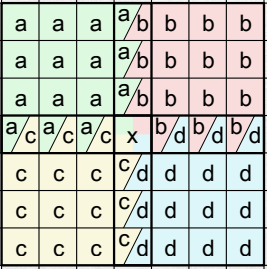
\includegraphics[scale=0.8]{filter.png}
    \caption{Kuwahara filter}
    }
\end{figure}

Apply Kuwahara filter to color images such as RGB is not ideal. The main problem because of each channels will have different standard deviation which make the pixel can't decide the best regions for decide the pixel value. Therefor, the image will be convert to HSV. The brightness of each regions is calculated to choose which is the color used to determine which channel will be taken.\\


\textbf{Hardware} the project environment is CPU: Intel Core i7-7720HQ and GPU: NVIDIA GEFORCE GTX 1050 using Window subsystem linux.



\section{Implementation}
The labwork can be concluded in the following step:
\begin{itemize}
    \item Load an RGB image into a 3-Dim array
    \item Convert RGB image into a HSV image: Follow the work flow of labwork 8. First we convert the dimension from 0 to 255 into 0 to 1. Using function in figure below to determine how red, green, blue value change to h,s,v.
    \item Fine-art Transformation by apply Kuwahara filter to the image
\end{itemize}

\begin{figure}[H]
    \center{
        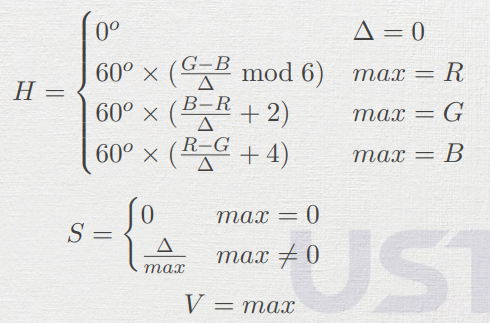
\includegraphics[scale=0.5]{hsv.png}
    \caption{Convert formula}
    }
\end{figure}

The following pictures are the base RGB image and the HSV images converted with GPU. The image shape are (634, 640, 3)

\begin{figure}[H]
    \center{
        
\includegraphics[scale=0.5]{lechonk.jpg}
    \caption{Sample image}
    }
\end{figure}

\begin{figure}[H]
    \center{
        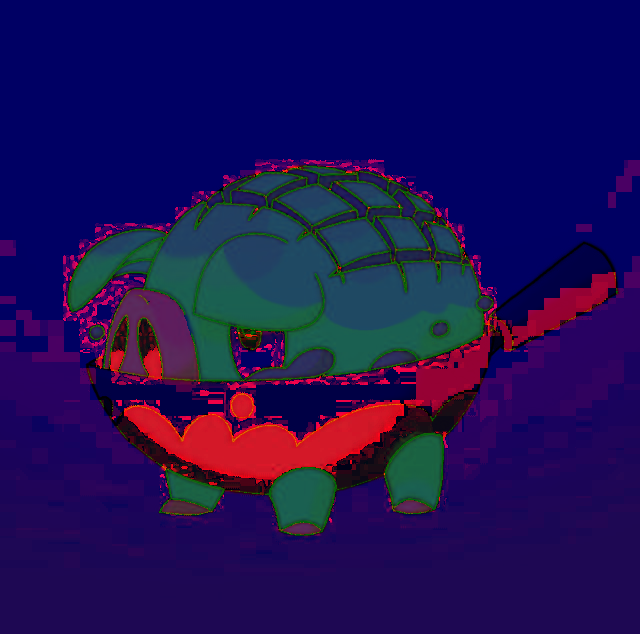
\includegraphics[scale=0.5]{HSV_lab10.png}
    \caption{HSV image converted with CPU}
    }
\end{figure}

\paragraph{HSV convert:} The following function is the code to convert the image from RGB to HSV
\begin{lstlisting}[language=Python]
@cuda.jit
def rgb_hsv(src, dst):
    tidx = cuda.threadIdx.x + cuda.blockIdx.x * cuda.blockDim.x
    tidy = cuda.threadIdx.y + cuda.blockIdx.y * cuda.blockDim.y
    r = src[tidx, tidy, 0]/255
    g = src[tidx, tidy, 1]/255
    b = src[tidx, tidy, 2]/255
    Max = max(r,g,b)
    Min = min(r,g,b)
    delta = Max - Min
    if delta == 0:
        h = 0
    elif Max == r:
        h = (60*(((g - b) / delta) % 6))
    elif Max == g:
        h = (60*(((b - r) / delta) + 2))
    elif Max == b: 
        h = (60*(((r - g) / delta) + 4))
    if Max == 0:
        s = 0
    if Max != 0:
        s = delta/ Max
    v = Max
    dst[tidx, tidy, 0] = h %360
    dst[tidx, tidy, 1] = s *100  
    dst[tidx, tidy, 2] = v *100
\end{lstlisting}

\paragraph{Kuwahara filter} 

\begin{figure}[H]
    \center{
        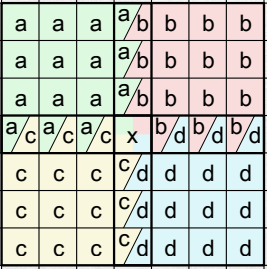
\includegraphics[scale=0.8]{filter.png}
    \caption{Kuwahara filter}
    }
\end{figure}
After the image convert to HSV, we apply the kuwahara filter to the RGB image with using brightness value of the hsv image.
The code below used to find the standard deviation of the regions of each pixels. And after we get the standard deviation of all 4 regions of a pixel, we will find the regions with minimum standard deviation and apply the value to the image
\begin{lstlisting}[language=Python]
@cuda.jit
    sum = 0
    sum2 = 0
    for i in  range(*sizes[0][0]):
        for j in range(*sizes[1][0]):
                sum = sum + (v[i,j])
                sum2 = sum2 + (v[i,j] * v[i,j])
    stadev1 = math.sqrt(sum2 / (size **2) - (sum / (size **2)) **2)
    ...
    for j in range(4):
        if Min == stadev[j]:
            temp = j
        for i in range(4):
            for wi in (sizes[temp][0]):
                for wj in (sizes[temp][1]):
                    r = r + src[wi,wj,2]
                    g = g + src[wi,wj,1]
                    b = b + src[wi,wj,0]
\end{lstlisting}

\begin{figure}[H]
    \center{
        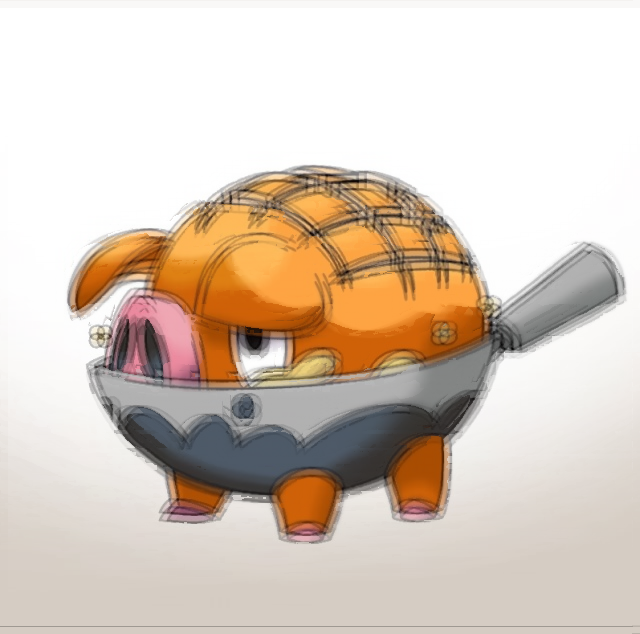
\includegraphics[scale=0.8]{kuwa.png}
    \caption{Image with kuwahara filter applied}
    }
\end{figure}

\paragraph{Discussion :} Apply Kuwahara filter with shared memory and with CPU are still work in progress. The kuwahara filter is applied without using shared memory.

\end{document}